\documentclass[../Orator]{subfiles}
\begin{document}

The FitzHugh-Nagumo model can be written in many ways, one of which is as follows.

\begin{equation}
    \dot{V}=V-\frac{V^{3}}{3}-W+I
\end{equation}

\begin{equation}
    \dot{W}=\phi (V+a-bW)
\end{equation}

The original values for the constants are \(a=0.7\), \(b=0.8\), and \(\phi=0.08\) \cite{}. For these values, the nullclines look like \Cref{fig:nullclines-original}. 

\begin{figure}[h]
    \centering
    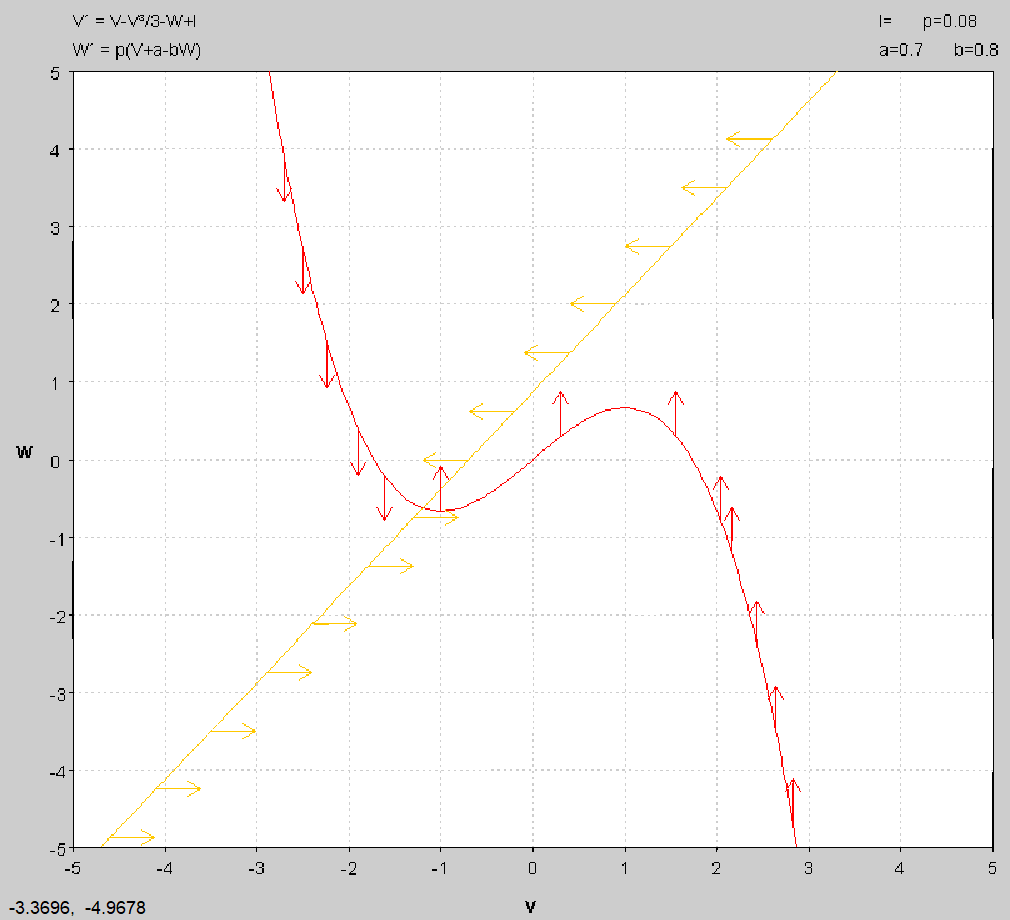
\includegraphics[width=400pt]{Pictures/Alex/Nullclines - original.PNG}
    \caption{Nullclines for \(I=0\), \(a=0.7\), \(b=0.8\), and \(\phi=0.08\)}
    \label{fig:nullclines-original}
\end{figure}

As can be seen in \Cref{fig:nullclines-original} there is only one equilibrium. This is located at \((-1.1994, -0.62426)\). This is a spiral sink. 

It is also possible for the model to have three equilibria. This is for example the case if \(b\) is changed to \(-0.8\). This can be seen in \Cref{fig:nullclines-negative}.

\begin{figure}[h]
    \centering
    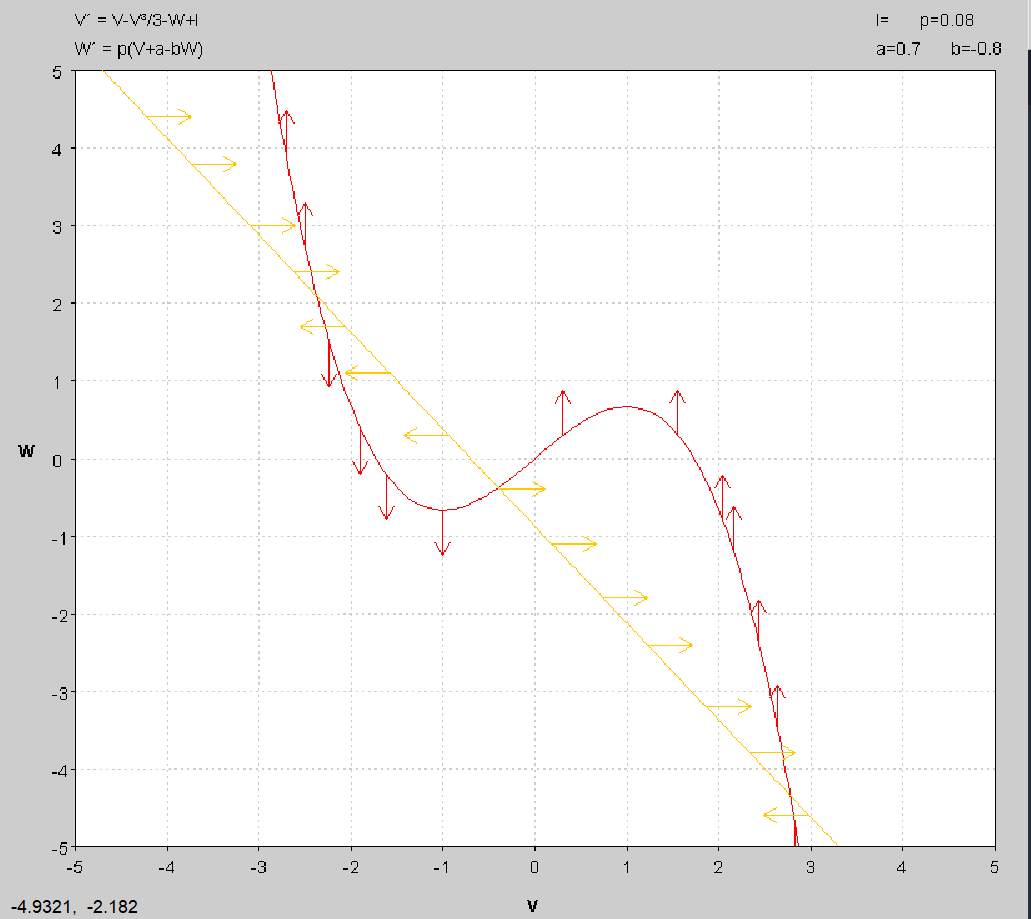
\includegraphics[width=400pt]{Pictures/Alex/Nullclines - negative.PNG}
    \caption{Nullclines for \(I=0\), \(a=0.7\), \(b=-0.8\), and \(\phi=0.08\)}
    \label{fig:nullclines-negative}
\end{figure}

Here the equilibria are at \((-2.376, 2.0949)\), \((-0.39825, -0.37719)\), and \((2.7742, -4.3428)\). The first and last are saddle points and the middle is a nodal source.

This change from one to three equilibria changes at b>0. 

\begin{comment}
    For Thursday:
    
    Parametric solutions: General solution based on the parameters.
    Why do we have 1/3 fixed points?
        Because of the slope of W???
        But why in a biological sense?
\end{comment}

\end{document}